\chapter{Исследовательский раздел}

В данном разделе приведены примеры идеального случая восстановления, среднего и плохого. Произведены исследования для определения времени обработки изображения в зависимости от радиуса дефокусировки и цветовой модели, а также полноты решения поставленной задачи. На основе полученных экспериментальных данных сделаны соответствующие выводы.

\section{Технические характеристики}

Технические характеристики машины, на которой производились исследования:

\begin{itemize}
	\item операционная система: Windows 10 64-bit;
	\item оперативная память: 16 Gb;
	\item процессор: AMD(R) Ryzen(TM) 5 4500U CPU @ 2.3 CHz;
	\item количество ядер: 8.
\end{itemize}

\section{Исследование времени работы предложенного метода в зависимости от размера изображения и цветовой модели}

\subsection*{Постановка исследования}

Исследование заключается в определении времени обработки изображения в зависимости от двух факторов: его размера и цветовой модели (трехканальная цветовая RGB~--~модель или одноканальная серая (англ. Grayscale) модель). 

Для замеров должны быть использованы дефокусированные изображения различных размеров и пропорций. Замеры необходимо провести несколько раз для минимизации влияния случайных факторов.

Гипотеза заключается в том, что графики зависимостей будут иметь линейный вид, а также время, затраченное на обработку цветного изображения, будет превышать время обработки одноканального изображения примерно в 3 раза.

\subsection*{Результаты исследования}

В таблице 4.1 представлены результаты замеров времени выполнения алгоритма в зависимости от размера исходного изображения и цветовой модели (RGB~--~модель или Grayscale). Размер изображения измеряется в пикселях, а время --- в секундах. Для замеров времени выполнения использовались команды \textit{tic} и \textit{toc}, представленные в MatLAB.

\renewcommand{\arraystretch}{1.5}
\begin{table}[h!]
	\begin{center}
		\caption{Зависимость времени обработки изображения от его размера и цветовой модели}
		""\newline
		\label{tabl}
		\begin{tabular}{ |c|c|c| } 
			\hline
			\textbf{Размер изображения}, (Ш $\times$ В, пиксели) & \textbf{RGB}, сек. & \textbf{Grayscale}, сек.\\
			\hline
			300 $\times$ 300 & 4.45 & 1.5\\
			\hline
			300 $\times$ 500 & 10.29 & 3.26\\
			\hline
			400 $\times$ 400 & 10.23 & 2.94\\
			\hline
			500 $\times$ 500 & 16.96 & 4.70\\
			\hline
			300 $\times$ 900 & 17.07 & 5.84\\
			\hline
			600 $\times$ 600 & 20.48 & 6.87\\
			\hline
			500 $\times$ 900 & 29.76 & 10.06\\
			\hline
			700 $\times$ 700 & 28.07 & 9.74\\
			\hline
			500 $\times$ 1200 & 40.29 & 13.39\\
			\hline
			700 $\times$ 900 & 42.53 & 14.06\\
			\hline
			800 $\times$ 800 & 37.09 & 13.07\\
			\hline
			900 $\times$ 900 & 49.67 & 16.52\\
			\hline
			700 $\times$ 1200 & 57.75 & 19.35\\
			\hline
			1000 $\times$ 1000 & 62.09 & 20.59\\
			\hline
			1100 $\times$ 1100 & 77.00 & 27.06\\
			\hline
			1200 $\times$ 1200 & 93.28 & 32.32\\
			\hline
		\end{tabular}
	\end{center}
\end{table}

\clearpage

На рисунке \ref{speed} представлена зависимость времени обработки изображения от количества пикселей и используемой цветовой модели.

\begin{figure}[!h]
	\centering
	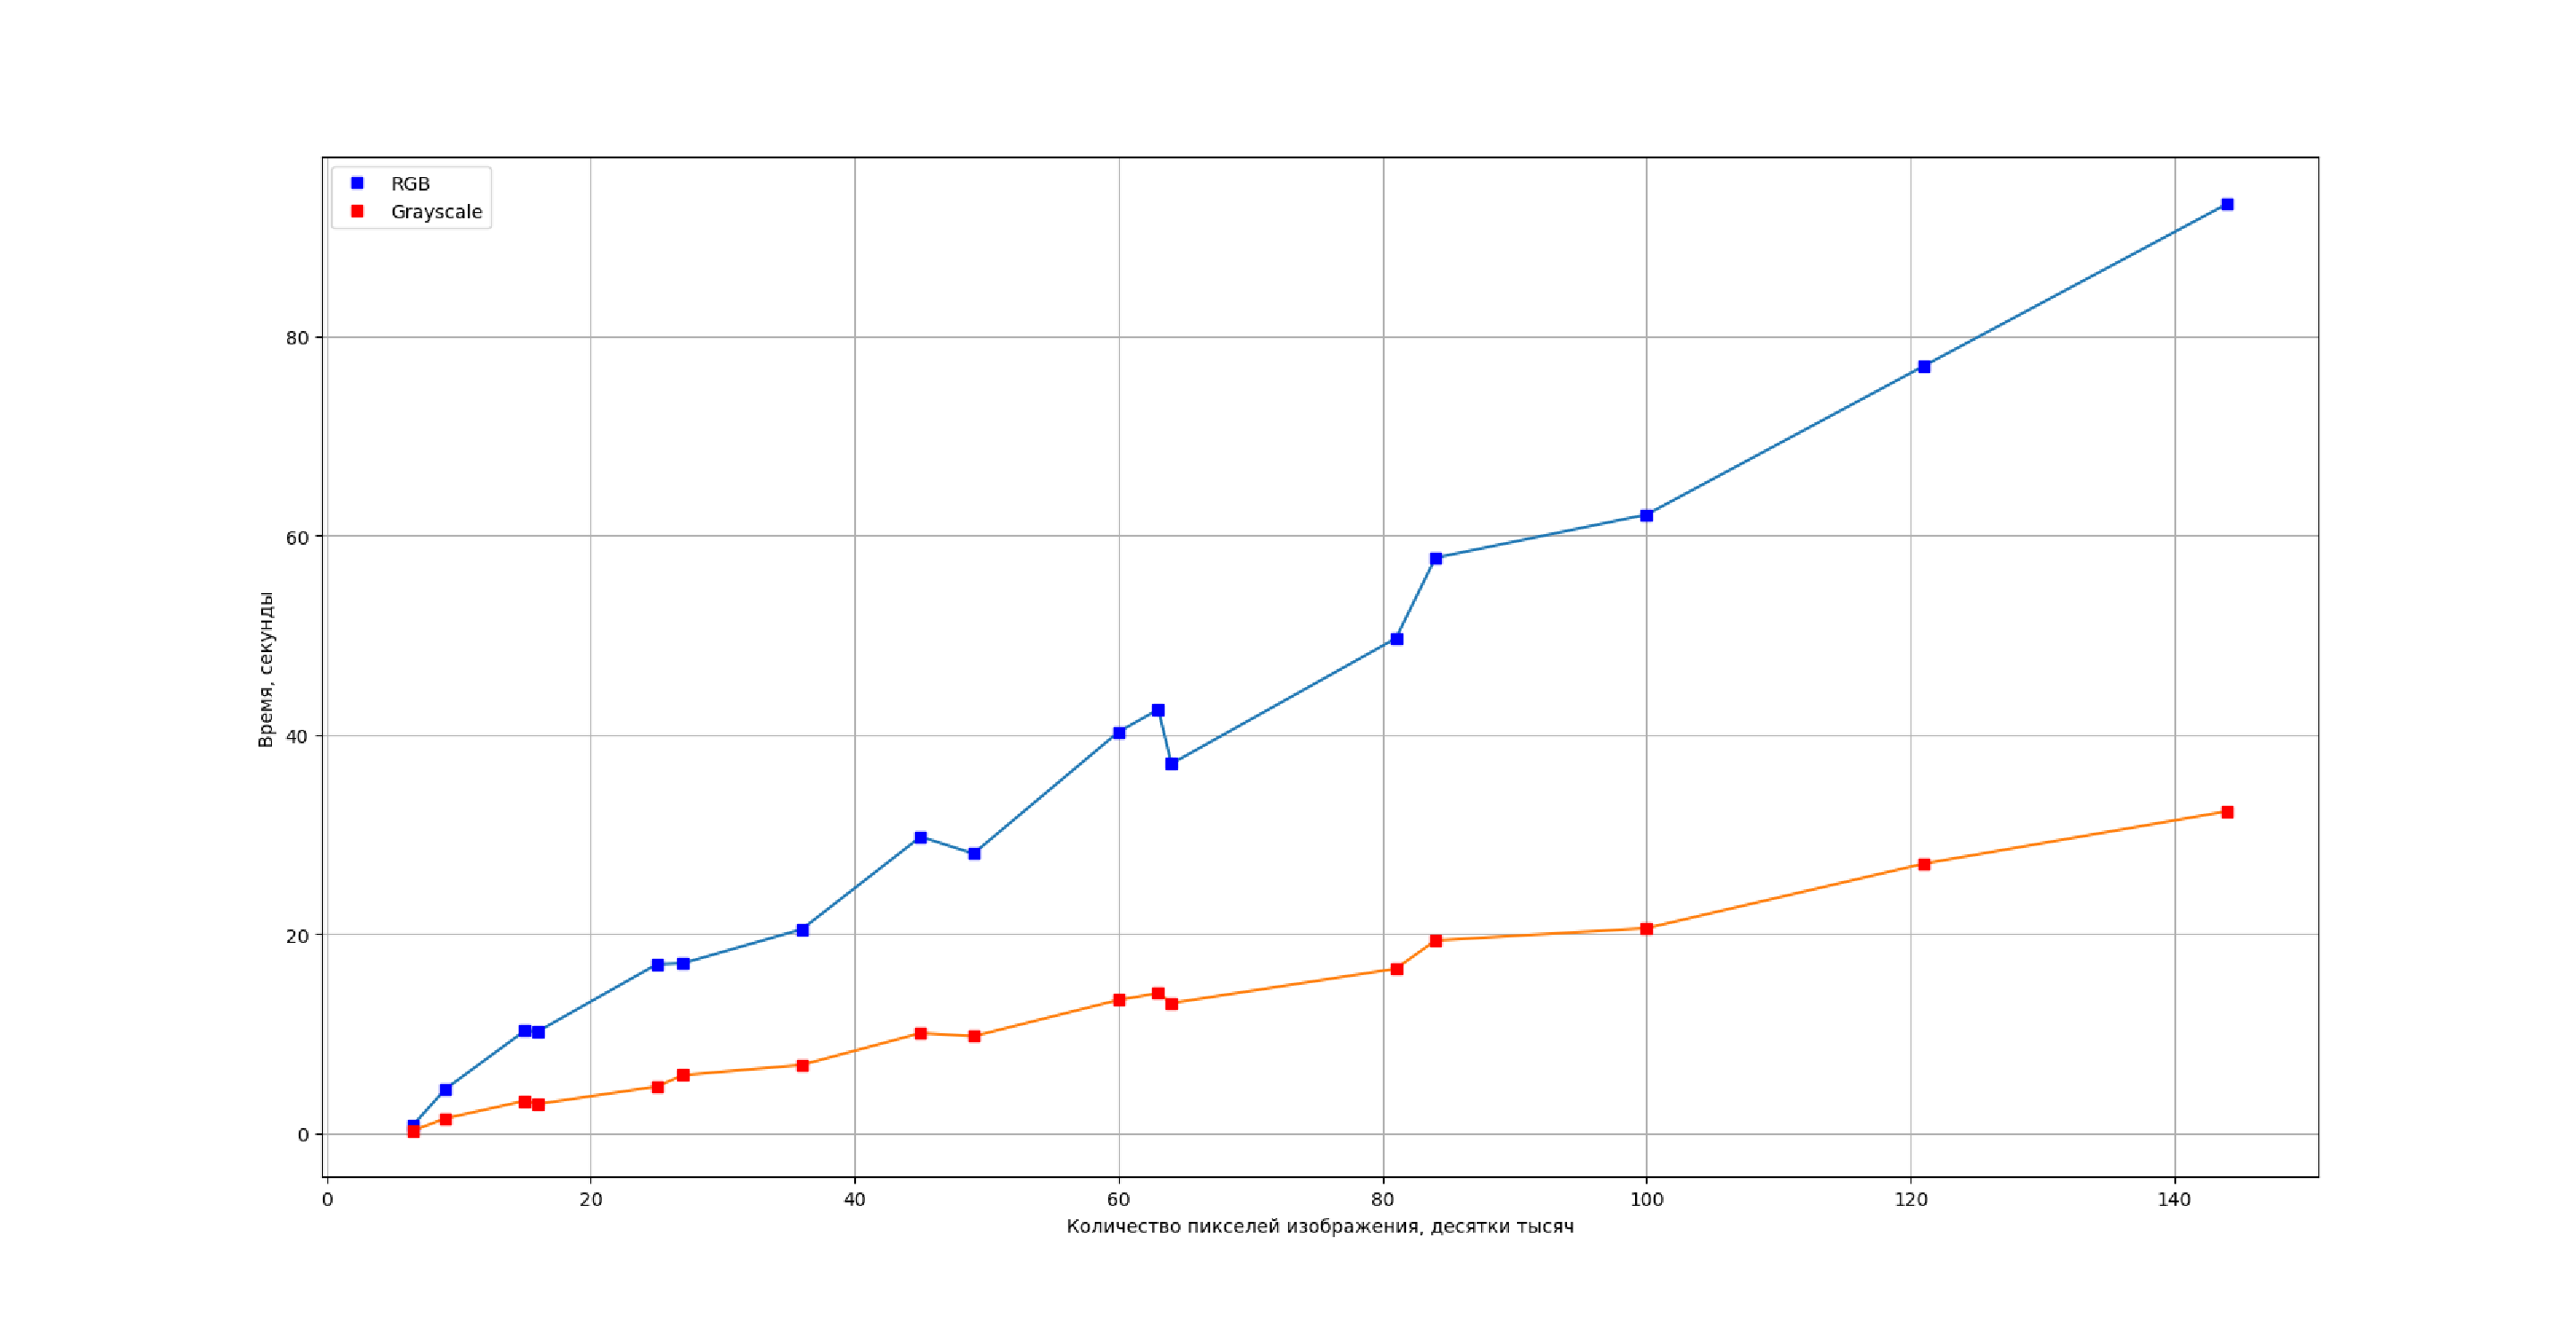
\includegraphics[scale=0.37]{assets/speed}
	\caption{Зависимость времени обработки изображения от количества пикселей и цветовой модели}
	\label{speed}
\end{figure}

Гипотеза подвердилась --- график зависимости имеет линейный вид, а также обработка цветных изображений требует примерно в 3 раза больше времени, чем обработка одноканальных изображений, что подтверждает линейность работы алгоритма относительно аддитивной цветовой модели. 

Таким образом, если цветовая информация об изображении не является критической для рассмотрения, то рекомендуется использовать изображения в тонах серого, т.к. с точки зрения структуры изображения они содержат ту же информацию, однако обработка такого изображения может быть значительно быстрее.

\section{Исследование полноты решения поставленной задачи}

\subsection*{Постановка исследования}

Исследование заключается в определении точности вычисления (в процентах) радиуса дефокусировки в зависимости от его величины и цветовой модели (RGB~--~модель или одноканальная). Для замеров должны быть использованы дефокусированные изображения различных размеров и пропорций.

Гипотеза заключается в том, что при радиусе размытия, равном 0 или 1, точность будет низкая, т.к. на кепстре структуры практически не будут наблюдаться. 

При достижении определенного порогового значения радиуса, которое необходимо установить в результате эксперимента, точность восстановления снова станет низкой, т.к. кольца на структуре кепстра будут сконцентрированы ближе к центру, и, соответственно, будет сложно отличить границу кольца от шума вокруг центра. Между описанными двумя областями значений радиусов точность, по предположению, должна быть удовлетворительной. 

Также предполагается, что точность вычислений для RGB~--~модели будет ниже, чем для серой, т.к. цветные изображения могут быть более подвержены шумам, а также в виду корреляции между каналами и дополнительной сложности вычислений может происходить накопление ошибки.

\subsection*{Результаты исследования}

На рисунке \ref{full} представлена зависимость точности вычисления радиуса дефокусировки от его величины и цветовой модели. Для каждого радиуса размытия обрабатывался ряд изображений различного размера и пропорций, а результат усреднялся.

\begin{figure}[H]
	\centering
	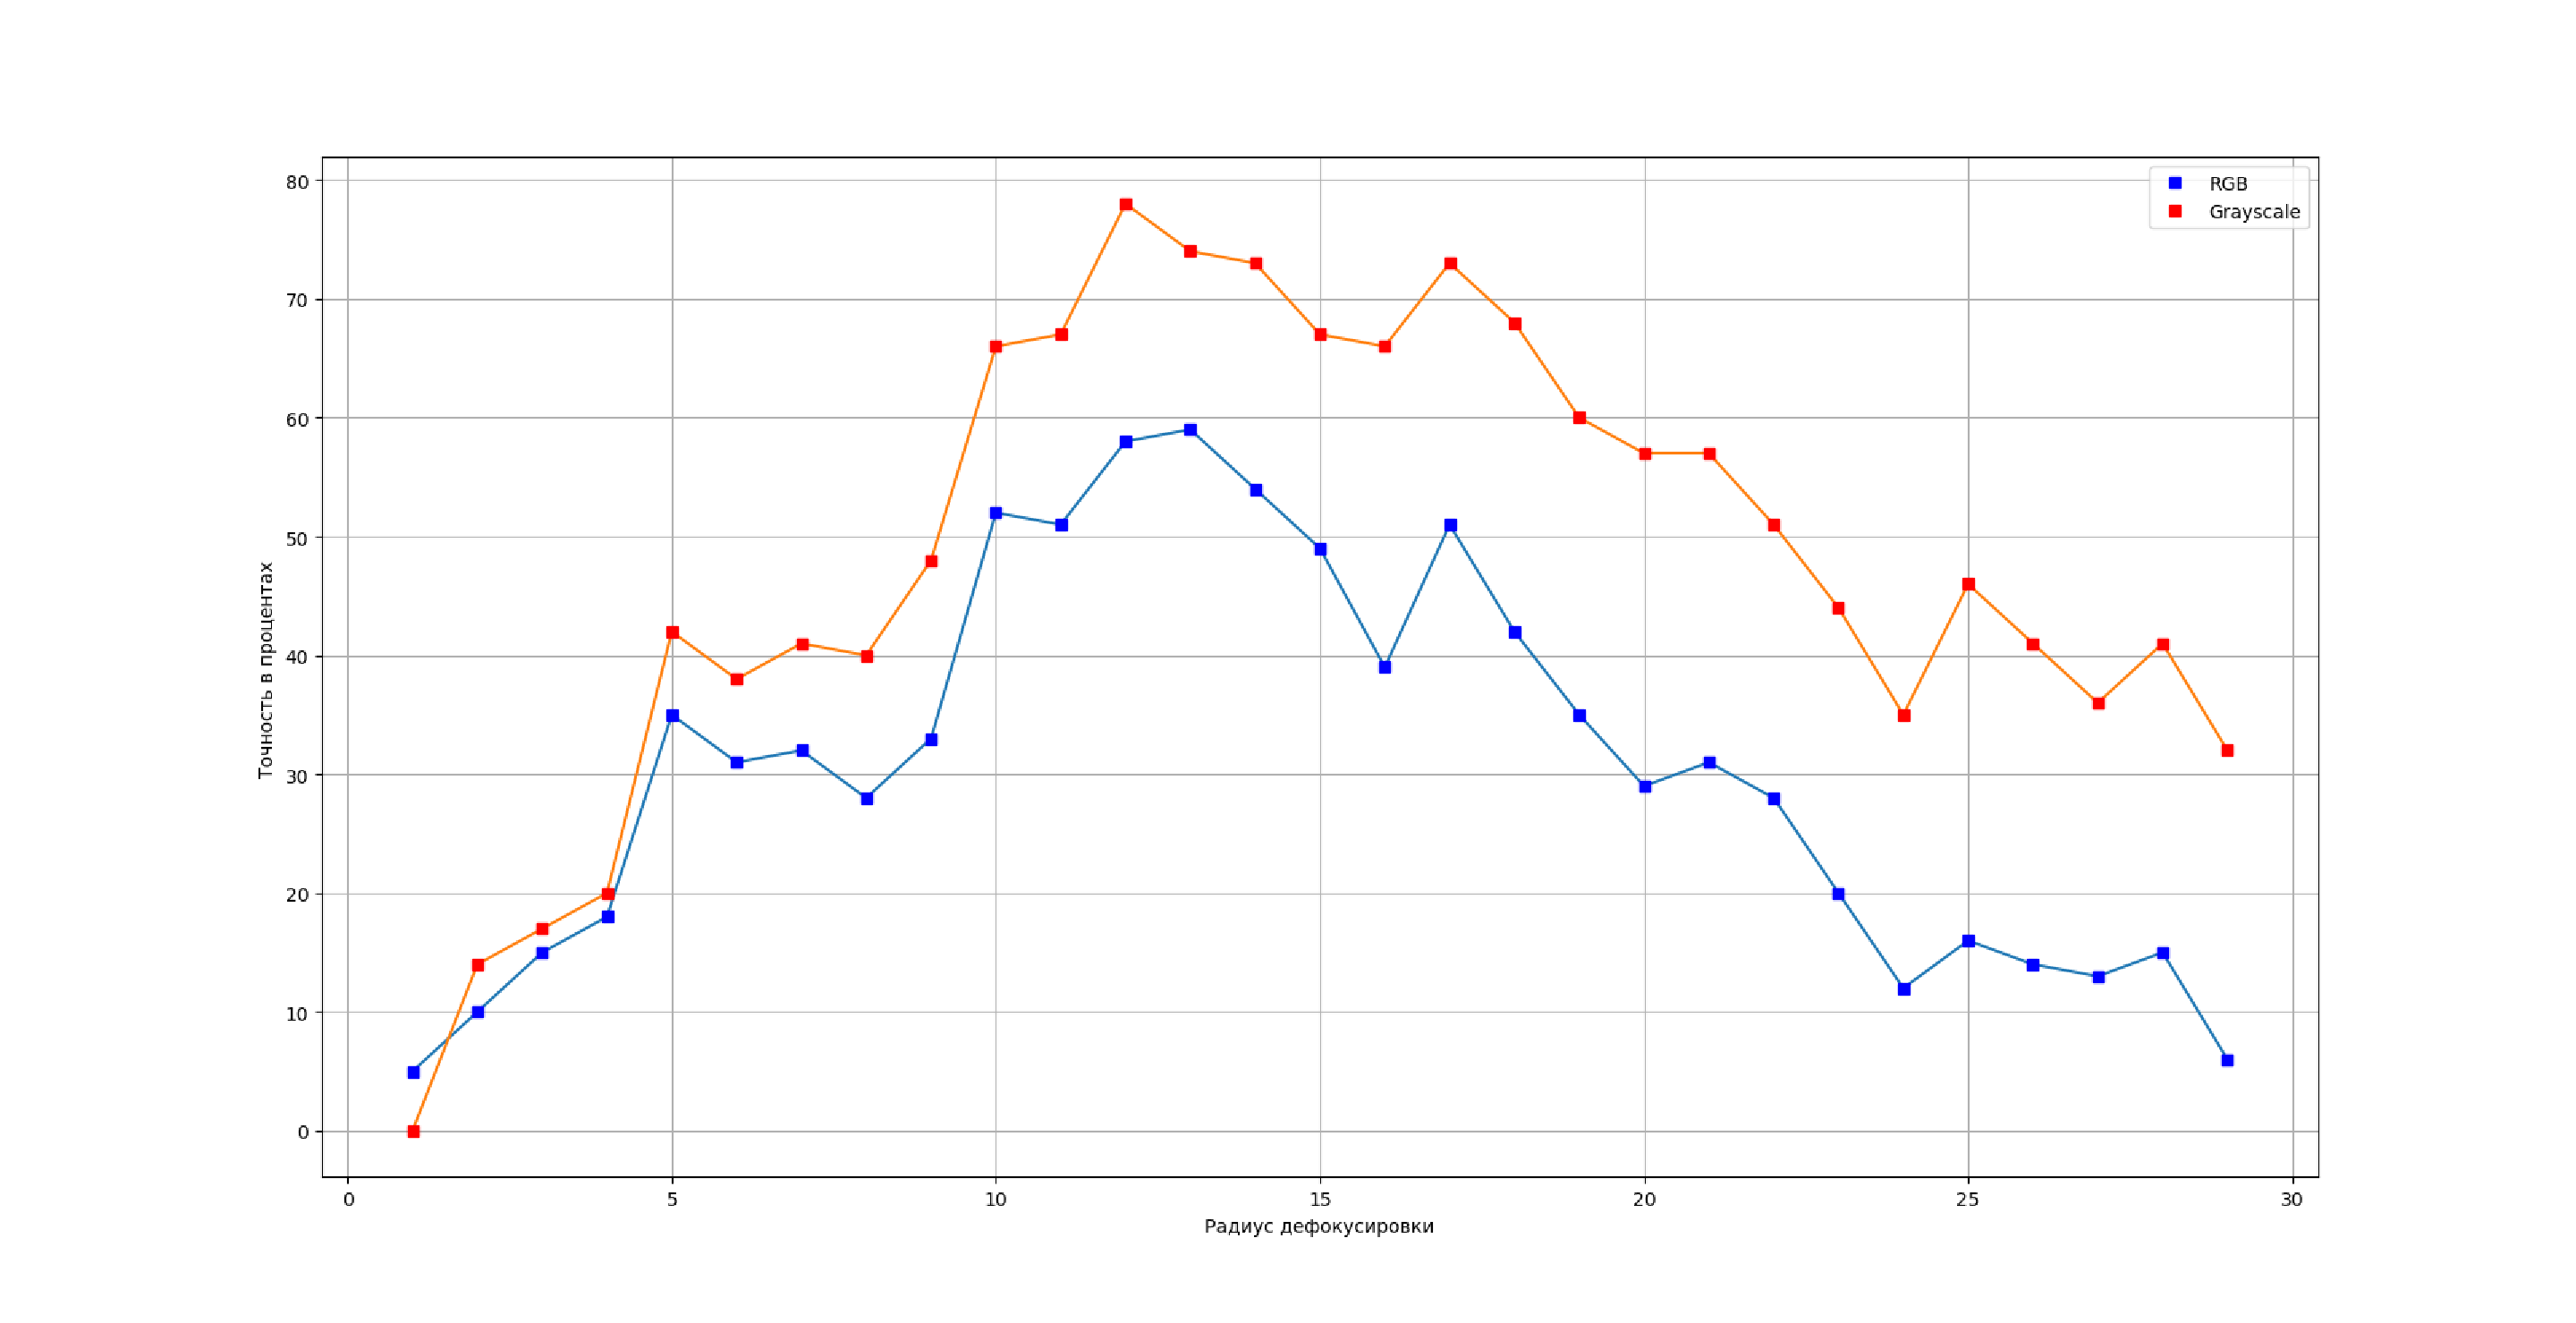
\includegraphics[scale=0.35]{assets/exp_accuracy}
	\caption{Зависимость точности вычисления радиуса дефокусировки от его величины и цветовой модели}
	\label{full}
\end{figure}

В таблице \ref{tabl} представлены результаты исследования полноты полученного решения.

\renewcommand{\arraystretch}{1.3}
\begin{table}[h!]
	\begin{center}
		\caption{Зависимость точности вычисления радиуса дефокусировки от его величины и цветовой модели}
		""\newline
		\label{tabl}
		\begin{tabular}{ |c|c|c| } 
			\hline
			\textbf{Радиус дефокусировки}, пиксели & \textbf{RGB}~--~модель & \textbf{Grayscale}~--~модель\\
			\hline
			0 & 0 \% & 0 \%\\
			\hline
			1 & 5 \%& 0 \%\\
			\hline
			2 & 10 \%& 14 \%\\
			\hline
			3 & 15 \%& 17 \%\\
			\hline
			4 & 18 \%& 20 \%\\
			\hline
			5 & 35 \%& 42 \%\\
			\hline
			6 & 31 \%& 38 \%\\
			\hline
			7 & 32 \%& 41 \%\\
			\hline
			8 & 28 \%& 40 \%\\
			\hline
			9 & 33 \%& 48 \%\\
			\hline
			10 & 52 \%& 66 \%\\
			\hline
			11 & 51 \%& 67 \%\\
			\hline
			12 & 58 \%& 78 \%\\
			\hline
			13 & 59 \%& 74 \%\\
			\hline
			14 & 54 \%& 73 \%\\
			\hline
			15 & 49 \%& 67 \%\\
			\hline
			16 & 39 \%& 66 \%\\
			\hline
			17 & 51 \%& 73 \%\\
			\hline
			18 & 42 \%& 68 \%\\
			\hline
			19 & 35 \%& 60 \%\\
			\hline
			20 & 29 \%& 57 \%\\
			\hline
			21 & 31 \%& 57 \%\\
			\hline
			22 & 28 \%& 51 \%\\
			\hline
			23 & 20 \%& 44 \%\\
			\hline
			24 & 12 \%& 35 \%\\
			\hline
			$\geq$25 & $\leq$20 \%& $\leq$40 \%\\
			\hline
		\end{tabular}
	\end{center}
\end{table}

Для определения точности восстановления в случае одноканальной модели была предложена следующая метрика:

\begin{equation}
	clean\_value = \cfrac{1 - |R_{calc} - R|}{R},
\end{equation}

\begin{equation}
	accuracy = 
	\begin{cases}
		0, & \text{если } clean\_value < 0 \text{ или } |clean\_value| > 1,\\
		clean\_value \cdot 100, & \text{иначе}.
	\end{cases}
\end{equation}

где $accuracy$ --- точность в процентах, $R_{calc}$ --- вычисленный радиус дефокусировки, $R$ --- реальный радиус. Для вычисления среднего значения для каждого радиуса использовалось значение $\cfrac{\sum_{i=1}^{N}accuracy_i}{N}$, где $N$ --- количество замеров. 

С случае оценки точности восстановления цветного изображения метрика $accuracy$ вычислялась для каждого канала независимо, а для получения среднего результата использовалось значение $\cfrac{\sum_{i=1}^{N}r\_accuracy_i\cdot g\_accuracy_i\cdot b\_accuracy_i}{N}$, где $r\_accuracy_i$, $g\_accuracy_i$, $b\_accuracy_i$ --- значение метрики i~--~го замера для красного, зеленого и синего цветовых каналов соответственно.

Таким образом, была определена область применимости предложенного метода: изображения с радиусом дефокусировки в диапазоне от 10 до 20 единиц. 

Если цветовая информация об изображении не является критической для рассмотрения, то рекомендуется использовать изображения в тонах серого, т.к. для этой цветовой модели точность вычислений выше.

\clearpage

\section{Демонстрация вариантов работы метода в зависимости от точности вычислений}

В связи с тем, что разрабатываемый метод основан на методе максимального правдоподобия, возможны несколько классов результатов восстановления: идеальный случай (реальный и вычисленный радиусы совпадают), средний (вычисление радиуса произошло с погрешностью) и плохой случай, когда реальный и вычисленный радиусы существенно не совпадают.

%На рисунке \ref{init} представлено исходное изображение, используемое для проведения эксперимента.
%
%\begin{figure}[H]
%	\centering
%	\includegraphics[scale=0.75]{assets/lena}
%	\caption{Исходное изображение, используемое для проведения эксперимента}
%	\label{init}
%\end{figure}

На рисунках \ref{expr7} и \ref{expr8} представлены примеры высокого (идеального) качества восстановления. Для проведения эксперимента были использованы изображения номера автомобиля~\cite{car} и кота~\cite{cat}.

\begin{figure}[!h]
	\centering
	\begin{subfigure}{.5\textwidth}
		\centering
		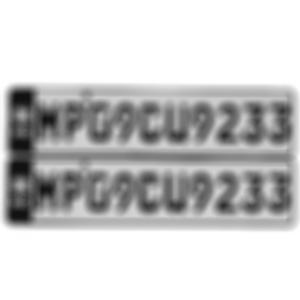
\includegraphics[scale=0.65]{assets/car_perfect}
	\end{subfigure}%
	\begin{subfigure}{.5\textwidth}
		\centering
		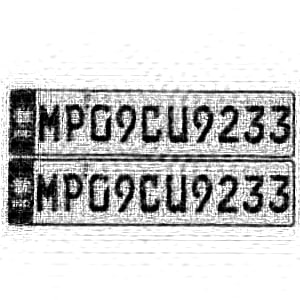
\includegraphics[scale=0.85]{assets/car_perfect_result}
	\end{subfigure}
	\caption{Пример восстановления высокого качества}
	\label{expr7}
\end{figure}

\begin{figure}[!h]
	\centering
	\begin{subfigure}{.5\textwidth}
		\centering
		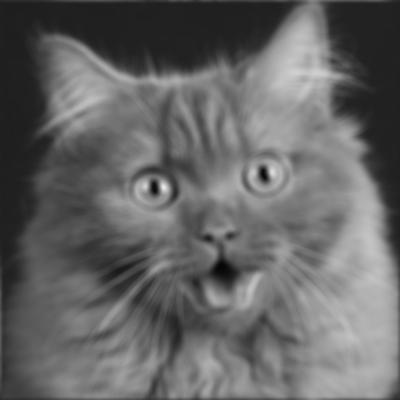
\includegraphics[scale=0.45]{assets/cat_perfect}
	\end{subfigure}%
	\begin{subfigure}{.5\textwidth}
		\centering
		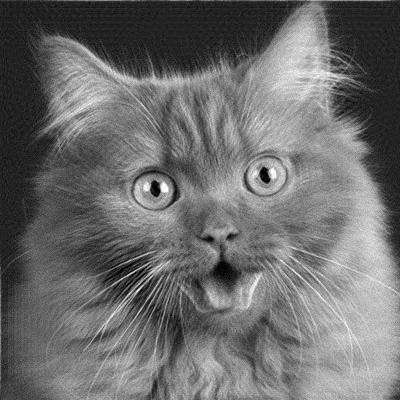
\includegraphics[scale=0.46]{assets/cat_perfect_result}
	\end{subfigure}
	\caption{Пример восстановления высокого качества}
	\label{expr8}
\end{figure}

\clearpage

Пиковое отношение сигнал~--~шум для первой пары изображений составляет 14.7 дб, для второй --- 23 дб.

На рисунках \ref{expr5} и \ref{expr6} представлены примеры среднего качества восстановления. Точность вычисления радиуса дефокусировки составляет $\approx$ 80 процентов.

\begin{figure}[!h]
	\centering
	\begin{subfigure}{.5\textwidth}
		\centering
		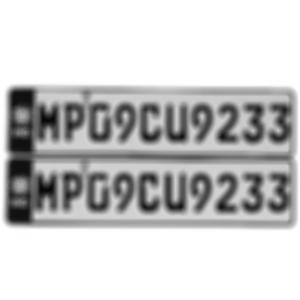
\includegraphics[scale=0.65]{assets/car_r5}
	\end{subfigure}%
	\begin{subfigure}{.5\textwidth}
		\centering
		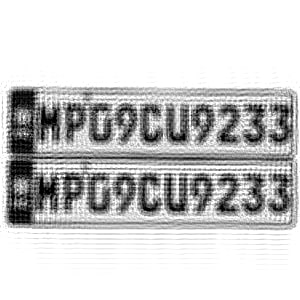
\includegraphics[scale=0.85]{assets/car_r5_result}
	\end{subfigure}
	\caption{Пример восстановления среднего качества}
	\label{expr5}
\end{figure}

\begin{figure}[!h]
	\centering
	\begin{subfigure}{.5\textwidth}
		\centering
		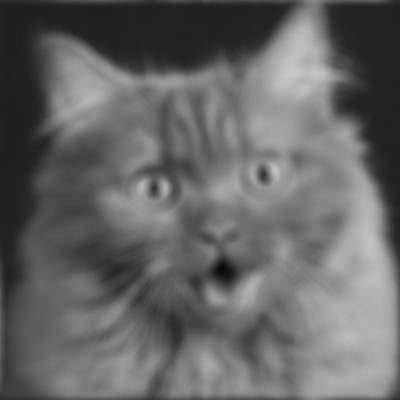
\includegraphics[scale=0.5]{assets/cat_norm}
	\end{subfigure}%
	\begin{subfigure}{.5\textwidth}
		\centering
		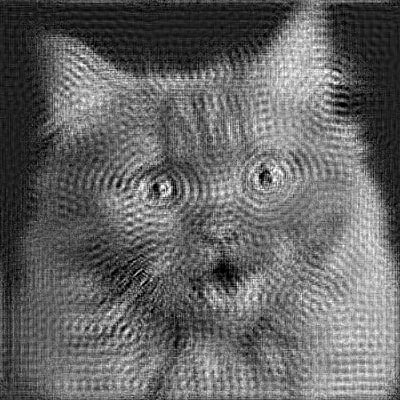
\includegraphics[scale=0.66]{assets/cat_norm_result}
	\end{subfigure}
	\caption{Пример восстановления среднего качества}
	\label{expr6}
\end{figure}

Пиковое отношение сигнал~--~шум для первой пары изображений составляет 19.5 дб, для второй --- 20.22 дб.

\clearpage

На рисунках \ref{expr9} и \ref{expr10} представлены примеры низкого качества восстановления. Точность вычисления радиуса дефокусирвоки составляет $\approx$70 процентов.

\begin{figure}[!h]
	\centering
	\begin{subfigure}{.5\textwidth}
		\centering
		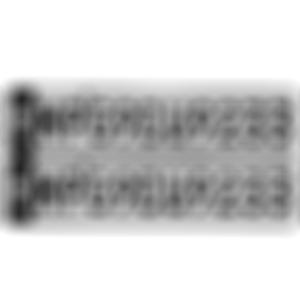
\includegraphics[scale=0.65]{assets/car_bad}
	\end{subfigure}%
	\begin{subfigure}{.5\textwidth}
		\centering
		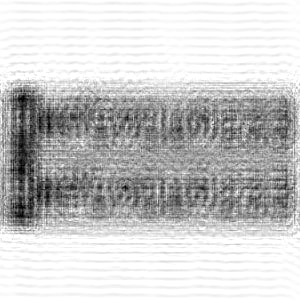
\includegraphics[scale=0.85]{assets/car_bad_result}
	\end{subfigure}
	\caption{Пример восстановления низкого качества}
	\label{expr9}
\end{figure}

\begin{figure}[!h]
	\centering
	\begin{subfigure}{.5\textwidth}
		\centering
		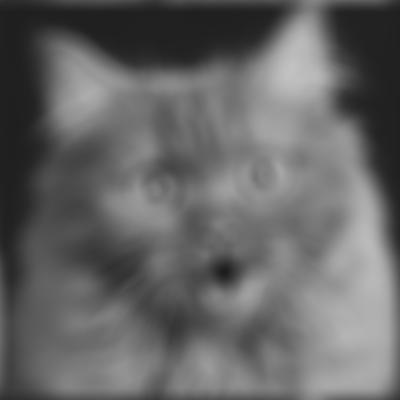
\includegraphics[scale=0.5]{assets/cat_bad}
	\end{subfigure}%
	\begin{subfigure}{.5\textwidth}
		\centering
		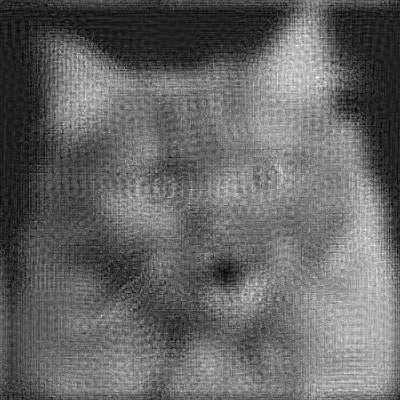
\includegraphics[scale=0.66]{assets/cat_bad_result}
	\end{subfigure}
	\caption{Пример восстановления низкого качества}
	\label{expr10}
\end{figure}

Пиковое отношение сигнал~--~шум для первой пары изображений составляет 21.9 дб, для второй --- 23.8 дб.
%
%\section{Исследование работы метода в случае замыкания}
%
%\subsection*{Постановка эксперимента}
%
%Эксперимент заключается в попытке повторного восстановления изображения, т.е. рассматривается ситуация, когда исходное изображение было для восстановления было получено в результате работы исследуемой программы.
%
%Гипотеза заключается в том, что качество восстановленного повторно изображения станет неудовлетворительным в виду того, что ФРТ для такого изображения будет составлена неверно. Также не будет накапливаться рекуррентная оценка в методе Люси~--~Ричардсона, что приведет к дополнительным артефактам на изображении.
%%, так как сам алгоритм предполагает порождение некоторых артефактов, что при повторном применении приведет к потере информации о деталях изображения и усилении шума
%
%\subsection*{Результаты эксперимента}
%
%На рисунке \ref{exp11} представлен результат первой итерации применения алгоритма.
%
%\begin{figure}[!h]
%	\centering
%	\begin{subfigure}{.5\textwidth}
%		\centering
%		\includegraphics[scale=0.5]{assets/cat_defocused}
%	\end{subfigure}%
%	\begin{subfigure}{.5\textwidth}
%		\centering
%		\includegraphics[scale=0.5]{assets/cat_restored}
%	\end{subfigure}
%	\caption{Результат первой итерации применения алгоритма}
%	\label{exp11}
%\end{figure}
%
%На рисунке \ref{exp12} представлен результат второй итерации применения алгоритма.
%
%\begin{figure}[!h]
%	\centering
%	\begin{subfigure}{.5\textwidth}
%		\centering
%		\includegraphics[scale=0.5]{assets/cat_restored}
%	\end{subfigure}%
%	\begin{subfigure}{.5\textwidth}
%		\centering
%		\includegraphics[scale=0.5]{assets/cat_repeat}
%	\end{subfigure}
%	\caption{Результат второй итерации применения алгоритма}
%	\label{exp12}
%\end{figure}
%
%Таким образом, гипотеза подтвердилась: при замыкании предложенного метода качество восстановления существенно ухудшается. При повторных попытках восстановить изображение методом <<слепой>> деконволюции его качество может ухудшаться по нескольким причинам, таким как накопление ошибки, несовершенство модели искажения, увеличение шума, усиление артефактов.
%
%\clearpage

%\section{Исследование работы предложенного метода в случае восстановления заведомо недефокусированного изображения}
%
%\subsection*{Постановка эксперимента}
%
%Эксперимент заключается в попытке восстановления заведомо недефокусированного изображения.
%
%Гипотеза заключается в том, что качество изображения станет неудовлетворительным.
%
%\subsection*{Результаты эксперимента}
%
%На рисунке \ref{exp12} представлен результат применения алгоритма к заведомо недефокусированному изображению.
%
%\begin{figure}[!h]
%	\centering
%	\begin{subfigure}{.5\textwidth}
%		\centering
%		\includegraphics[scale=0.55]{assets/text}
%	\end{subfigure}%
%	\begin{subfigure}{.5\textwidth}
%		\centering
%		\includegraphics[scale=0.75]{assets/text_restored}
%	\end{subfigure}
%	\caption{Результат применения алгоритма для недефокусированного изображения}
%	\label{exp2}
%\end{figure}
%
%Таким образом, гипотеза подтвердилась.

\section*{Выводы}

Было выявлено, что зависимость времени обработки изображения от его размера и цветовой модели имеет линейный вид, а обработка цветного изображения в среднем требует примерно в 3 раза больше времени, чем обработка серого. 

Была определена область применимости предложенного метода: в диапазоне радиуса дефокусировки от 10 до 20 единиц точность восстановления является удовлетворительный, а в случае обработки серого изображения этот диапазон еще шире, поэтому если учет информации о цвете изображения некритичен, то рекомендуется использовать серое изображение вместо цветного в целях сокращения времени обработки и повышения качества результата. Была описана метрика, используемая для оценки точности.

Были рассмотрены варианты работы программы: идеальный случай, нормальный и плохой, а также проведен анализ значения пикового отношения сигнал~--~шум для каждого варианта. Было выявлено, что метрика PSNR не всегда отражает действительное качество восстановления, т.к. не учитывает психофизиологические особенности восприянтия изображения человеком.